\chapter{Estado del Arte}
\label{cap:EstadoArte}

\setlength{\parindent}{0pt}

En este capítulo se explicará que es blockchain, como funciona, que tipos hay, así como ver su uso en el presente y que aplicaciones se están desarrollando alrededor de la misma para sacarle su máximo potencial, este apartado es de crucial importancia pues servirá para ver el estado del arte de las aplicaciones (en concreto aplicaciones móvil) del presente. Además, se explicará el trabajo realizado para preparar la aplicación móvil, en concreto la APIRestful que se ha desarrollado para comunicar el móvil con la base de datos y parte de la red blockchain. También, se estudian conceptos básicos de Android que se han aprendido para preparar el proyecto. 

% -------------------------------------------------- %
% -------------------------------------------------- %
\section{Blockchain}
Blockchain\cite{b1,b2,b3,b4} es un término escuchado hoy en día por todas partes, más a nivel económico que tecnológico. Y aunque pueda parecer complejo, su funcionamiento es bastante sencillo.

% -------------------------------------------------- %
\subsection{Definición}

Blockchain es una tecnología \textbf{DLT} (Distributed Ledger Tecnology), un \emph{ledger} es un libro contable o de contabilidad. Por lo que DLT viene a ser una tecnología de libros de contabilidad distribuidos. DLT se refiere a la infraestructura tecnológica y a los protocolos que permiten el \textbf{acceso, validación y actualización} de registros de forma \textbf{simultánea e inmutable} a través de una red que se extiende por \textbf{múltiples entidades} o ubicaciones (en el caso de blockchain, estas entidades son ordenadores y se les llama nodos). \\

La tecnología blockchain se sostiene en tres pilares principales:
\begin{enumerate}
  \item \textbf{Transparencia:} Toda la información que se registra en la red blockchain es pública, todas las transacciones pueden ser visualizadas por todos los nodos que conforman la red blockchain. Aunque pueda parecer peligroso que todo el mundo pueda ver todas las transacciones, Blockchain utiliza complejos mecanismos criptográficos para mantener el anonimato en la red, de modo que nunca se puede saber quienes son los participantes involucrados en una transacción. 
  \item \textbf{Inmutabilidad:} Una vez almacenada la información en la red, esta pasa a regirse por las reglas de la red, no pudiendo ser modificadas, alteradas o eliminadas de nunguna manera. 
  \item \textbf{Descentralización:} La información que registra la red blockchain no queda guardada en un único lugar, no hay una empresa con toda la información centralizada en sus instalaciones. Todos los nodos (ordenadores) que forman la red blockchain tienen una copia exacta y actualizada de la información que hay en la red. Las redes distribuidas permiten además eliminar la necesidad de una autoridad central que controle el sistema para evitar manipulaciones o fraudes. 
\end{enumerate}

\subsection{¿Como funciona?}

Una Blockchain es un sistema de registro de transacciones en constante crecimiento, junta la información en grupos conocidos como \textbf{bloques}. Cada bloque contiene información sobre las transacciones que se han realizado, así como información adicional en la cabecera. En la cabecera del bloque tenemos información sobre el número del bloque, el \textbf{hash} del bloque anterior, el \textbf{timestamp} y el \textbf{nonce} entre otros. \\

Entendamos estos conceptos:
\begin{itemize}
  \item Hash: Un hash\cite{whatIsHash} es un algoritmo que mezcla la información que se le introduce para generar una salida única e irreversible que tiene siempre una longitud fija. Es importante que cada salida es única para la información introducida, el más mínimo cambio en la información introducida y la salida cambiará por completo. Es como una huella digital de la información, no hay dos huellas iguales. Las funciones hash se utilizan de forma habitual para guardar la contraseña de personas en una base de datos, así, la contraseña nunca queda guardada en claro y si la base de datos se ve comprometida, es casi imposible recuperar la contraseña original \ref{fig:hash}. Aplicado a una red Blockchain, se ejecuta una función \textbf{hash256} sobre toda la información de un bloque. El resultado se utiliza en el siguiente bloque que se vaya a crear. Es decir, que cada bloque tiene el hash del bloque anterior (y el siguiente bloque tendrá el hash del bloque actual). 
  \item Timestamp: Identifica la hora exacta en segundos de la creación del bloque.
  \item Nonce: Un nonce\cite{whatIsNonce} es un número que solo puede ser utilizado una única vez. 
\end{itemize}

\begin{figure}[h!]
  \centering
  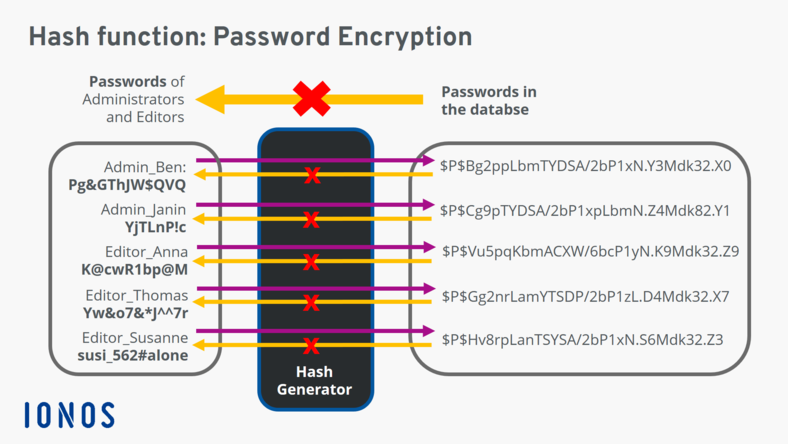
\includegraphics[width=0.8\linewidth]{figs/EstadoArte/Blockchain/hash}
  \caption[Ejemplo del hashing de una contraseña]{Ejemplo del hashing de una contraseña}
  \label{fig:hash}
\end{figure}

Para continuar con la explicación, utilizaremos redes blockchain que utilizan el algoritmo de consenso \textbf{Proof of Work}\cite{whatIsProofOfWork} como hace por ejemplo la red de \textbf{Bitcoin}\cite{whatIsBitcoin}. La base es la misma para la inmensa mayoría de redes, sin embargo según el algoritmo de consenso el método difiere ligeramente. Los algoritmos se verán mas adelante\ref{sec:Algor}. En el caso de Proof of Work, para añadir un nuevo bloque a la red, debe ser \textbf{minado}\cite{minarBitcoin}. Para minar un bloque, todos los nodos de la red blockchain tratan de encontrar un hash con un requisito añadido. Ejecutar un hash sobre cualquier tipo de información, es un proceso muy fácil. Por ello, utilizando Proof of Work, se añade una dificultad al hash. La dificultad\ref{fig:hashDiff} consiste en obligar que el hash resultante tenga un número de \textbf{0's} al principio del resultado. Por lo tanto, el minado consiste en modificar el \emph{nonce} (pues no se pueden modificar las transacciones que hay en el bloque o el hash del bloque anterior). Los nodos de la red modifican el nonce de forma aleatoria hasta que algún nodo logre dar con un nonce que cumpla con la dificultad del hash. Logrado esto, el resto de nodos de la red verifican que el nonce que ha encontrado resuelve en efecto la dificultad del hash y se procede a añadir el bloque a la red y vuelta a empezar. En el caso de bitcoin, se mina un bloque cada 10 minutos aproximadamente. \\

\clearpage

\begin{figure}[h!]
  \centering
  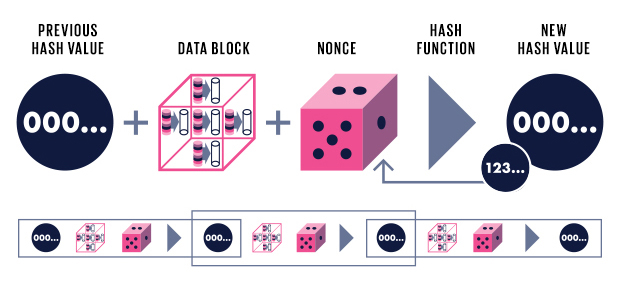
\includegraphics[width=0.9\linewidth]{figs/EstadoArte/Blockchain/hashDificultad}
  \caption[Hash dificultad]{Dificultad del hash}
  \label{fig:hashDiff}
\end{figure}

La vida de una transacción en bitcoin a grandes rasgos puede verse en la figura \ref{fig:bitcoin}. La razón de que blockchain sea una cadena de bloques, es que después de todo el proceso de hashing, de minado\dots los bloques quedan enlazados entre si gracias a estos hashes\ref{fig:bloqueEnlazado}. 

\begin{figure}[h!]
  \centering
  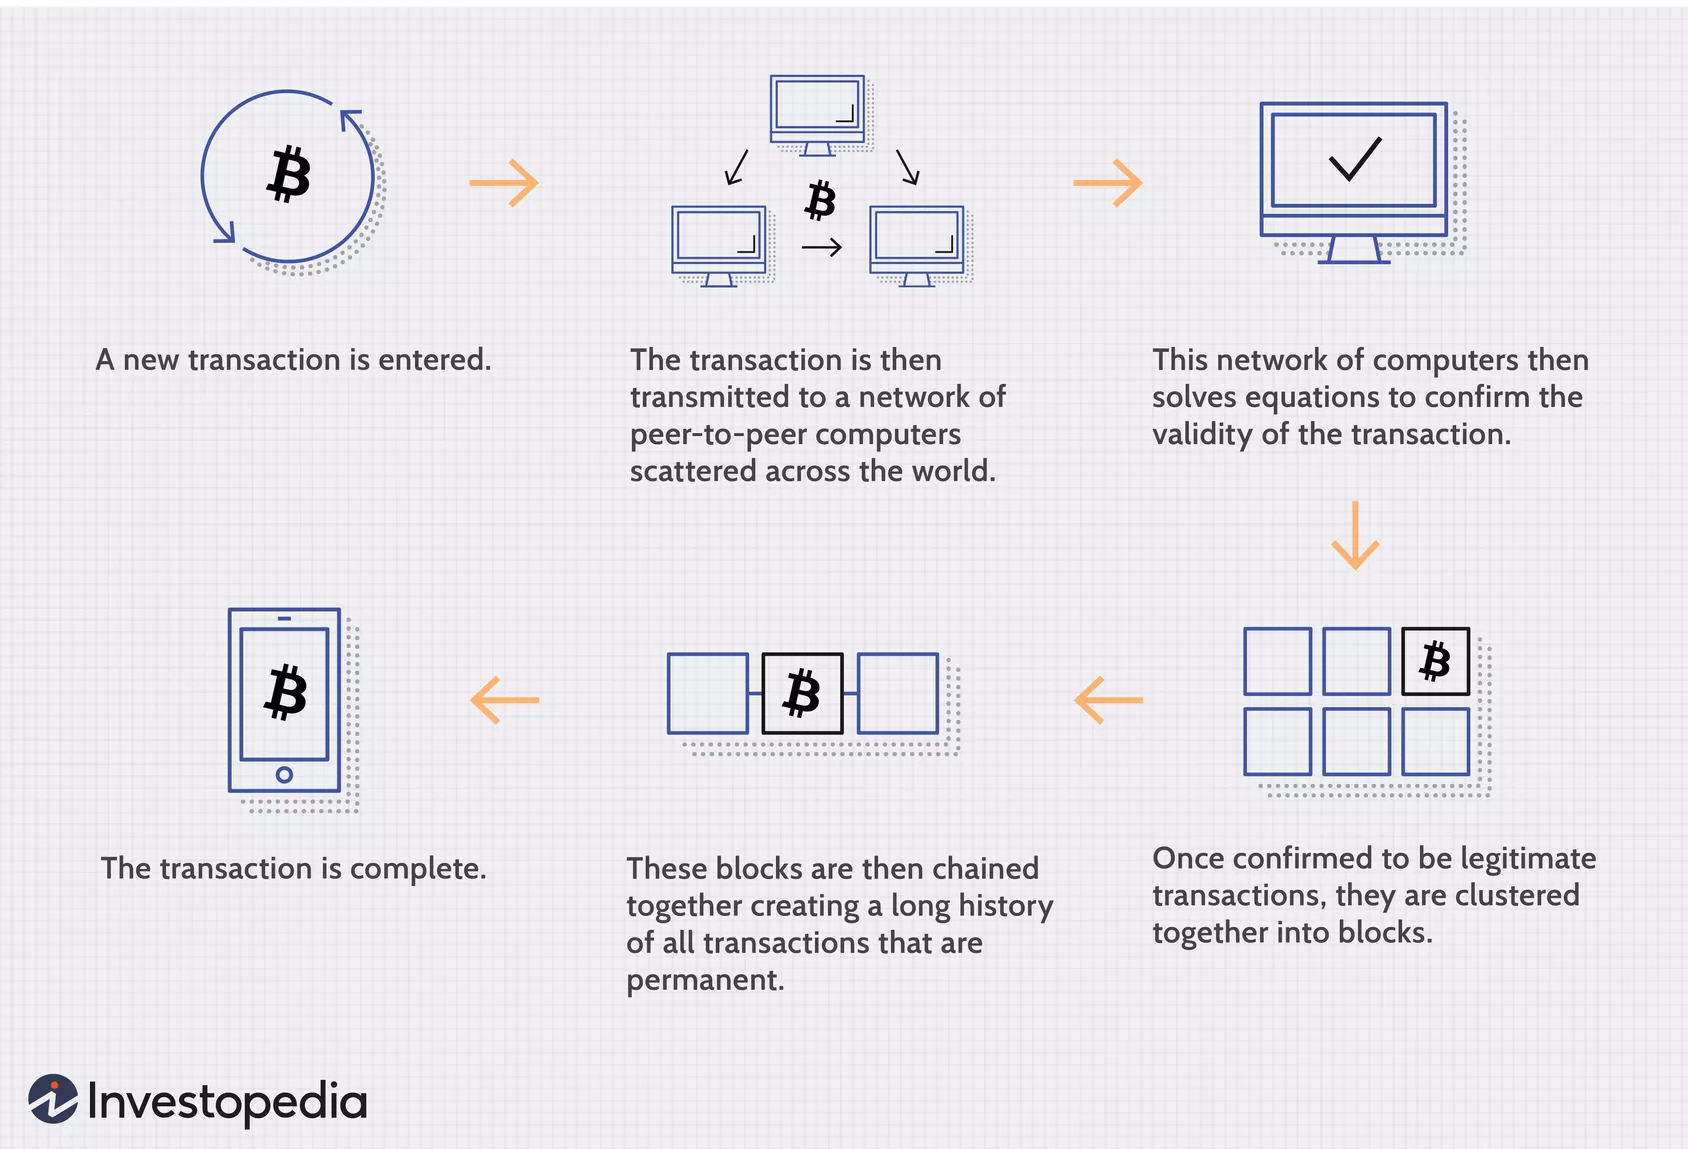
\includegraphics[width=0.9\linewidth]{figs/EstadoArte/Blockchain/bitcoinMining}
  \caption[Vida de una transacción en Bitcoin]{Vida de una transacción en Bitcoin}
  \label{fig:bitcoin}
\end{figure}

\begin{landscape}
\begin{figure}[h!]
  \centering
  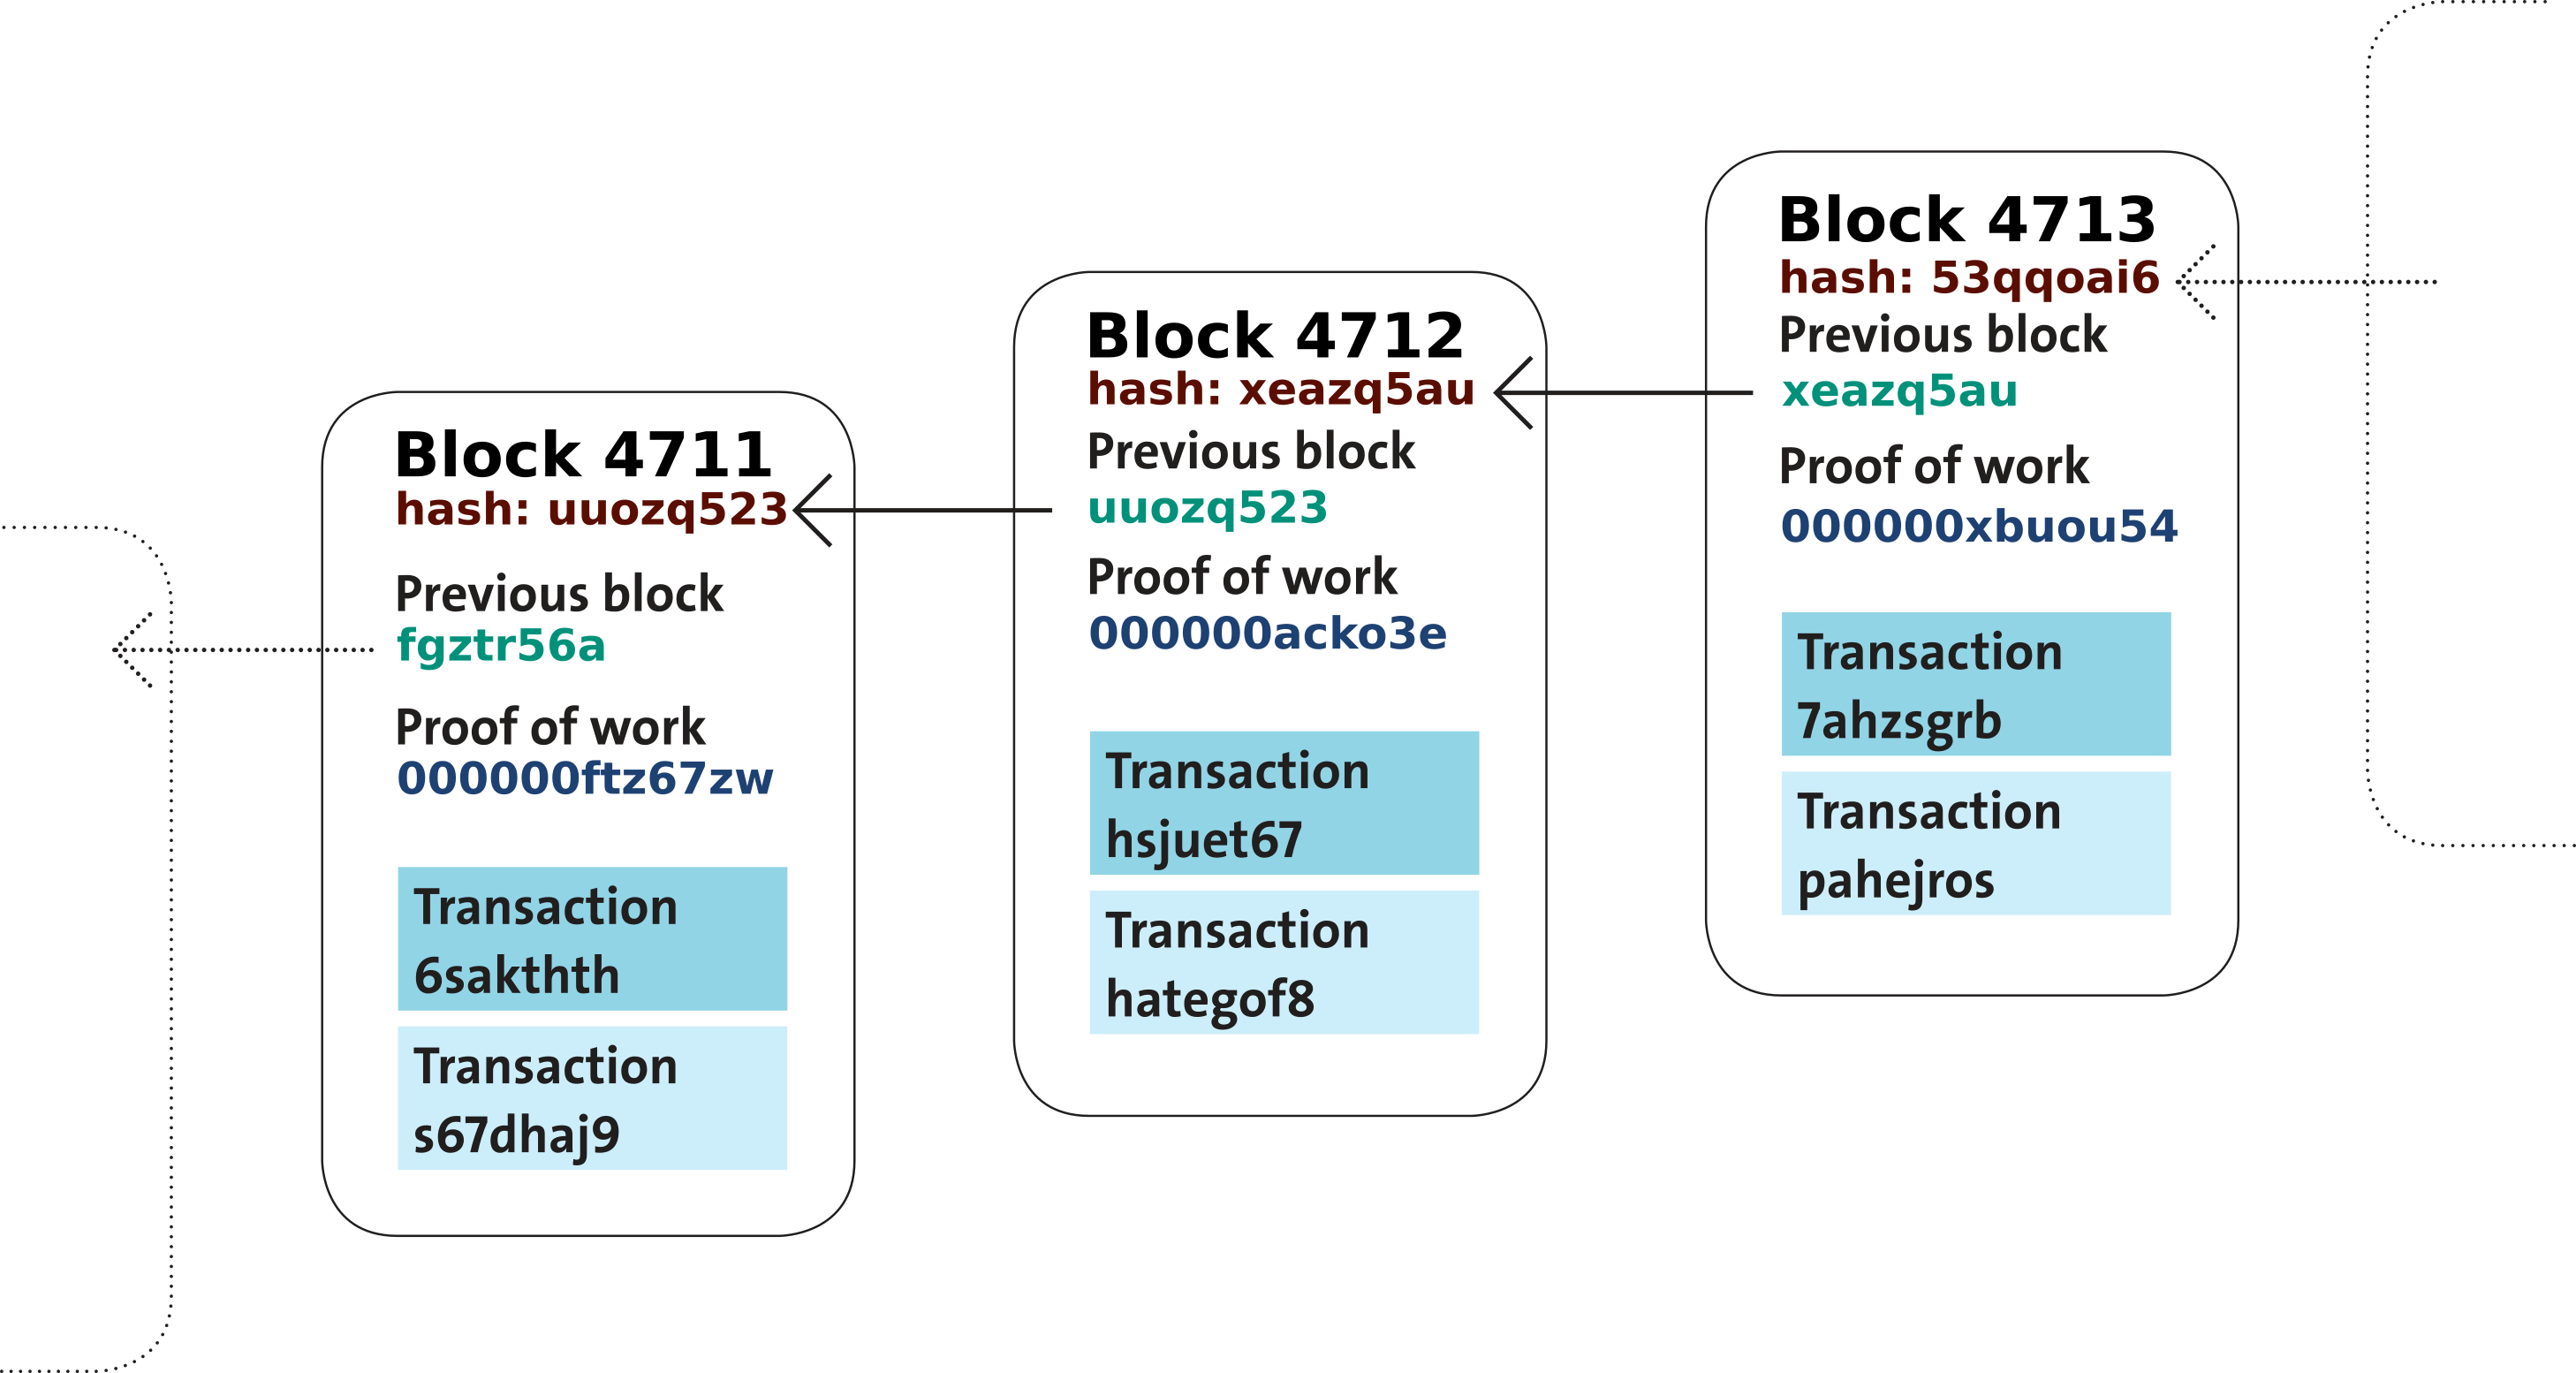
\includegraphics[width=0.8\linewidth]{figs/EstadoArte/Blockchain/bloqueEnlazado}
  \caption[Cadena de bloques]{Cadena de bloques}
  \label{fig:bloqueEnlazado}
\end{figure}
\end{landscape}

\clearpage
% -------------------------------------------------- %
\subsection{Tipos de redes blockchain}

Cuando se habla de blockchain, parece dar la impresión de que solo existe un tipo. Sin embargo hay varias redes con sus ventajas y desventajas\cite{tiposBlock1, tiposBlock2}. Las principales diferencias entre ellas son las \textbf{funcionalidades, protocolos de consenso, administración y reglas para validar las transacciones}.

\subsubsection{Blockchain pública}

Las blockchain públicas no tienen permisos, cualquier usuario es bienvenido a unirse a la red, a enviar transacciones, a utilizar las funcionalidades que tiene la red, y a minar bloques. Las principales características de esta red son:
\begin{itemize}
\item Son \textbf{transparentes}: El código, el funcionamiento interno, los smart contracts si tiene (se verá este término mas adelante) son todos públicos y de código abierto.
\item \textbf{Sin permisos}: Cualquier persona puede unirse a la red sin preguntar. Lo único que tiene que hacer es descargar la red y sincronizarse con los demás nodos.
\item Usuarios \textbf{anónimos} y \textbf{sin administradores}: Nadie se conoce en la red, se trabaja siempre con lo que se conoce como \textbf{address}, que viene a ser un identificador único por miembro dentro de la red para identificarlo. Además, no existe administrador de la red, no hay una persona o grupo que tenga poder sobre la red para hacer cambios de ningún tipo.
\item La información de la red puede ser \textbf{mantenida por todas las personas que lo deseen}. Y al minar nuevos bloques, dependiendo de la red, se ofrece un \textbf{incentivo}.
\end{itemize}

En resumidas cuentas, una blockchain pública es \emph{descentralizada}, \emph{distribuida}, \emph{consensuada}, \emph{abierta} y \emph{segura}. Algunos ejemplos de redes públicas son bitcoin\cite{webBitcoin} y ethereum\cite{webEthereum}

\subsubsection{Blockchain privada}

Las blockchains privadas son permisionadas, esto quiere decir que no cualquier persona puede añadirse como nodo libremente. Requieren de una \textbf{entidad} que ejerza de \textbf{administrador}. La mayoría de usuarios no consideran estas redes como blockchain a causa de esto mismo. El administrador de la red tiene que dar permiso a los usuarios para poder minar, enviar transacciones y participar en general en la red. \\

Además, es habitual que los datos estén almacenados en nodos centrales y no abiertos al público. Pudiendo acceder a los bloques de la red solo mediante invitación. \\

Algunos ejemplos de blockchains privadas son R3\cite{webR3}, Ripple\cite{webRipple} y Quorum\cite{webQuorum}

\subsubsection{Blockchain híbrida o federada}

Estas redes son utilizadas por grandes empresas y gobiernos, no tienen porqué estar abiertas al público, teniendo la gestión varias entidades. Además no tienen una criptomoneda asociada y no recompensan por el minado de bloques. Sin embargo el software que utilizan es de código abierto, como puede ser \textbf{Hyperldger, Corda}\cite{webHyper, webCorda}. \\

Como ejemplo tenemos la \emph{Enterprise Ethereum Alliance}, en la que participan el Banco Santander y BBVA. Esta red utiliza la blockchain de Ethereum (pública), sin embargo tienen su propia plataforma privada.

\subsubsection{Blockchain as a Service}

Estas redes blockchain son controladas por un proveedor de servicios como puede ser \emph{Amazon}. Estos proveedores permiten utilizar redes blockchain en la nube, permitiendo a los desarrolladores aprovechar el potencial de las redes blockchain sin la necesidad de invertir en el computo que ello requiere.

% -------------------------------------------------- %
\subsection{Tipos de algoritmo de consenso} \label{sec:Algor}

\begin{figure}[h!]
  \centering
  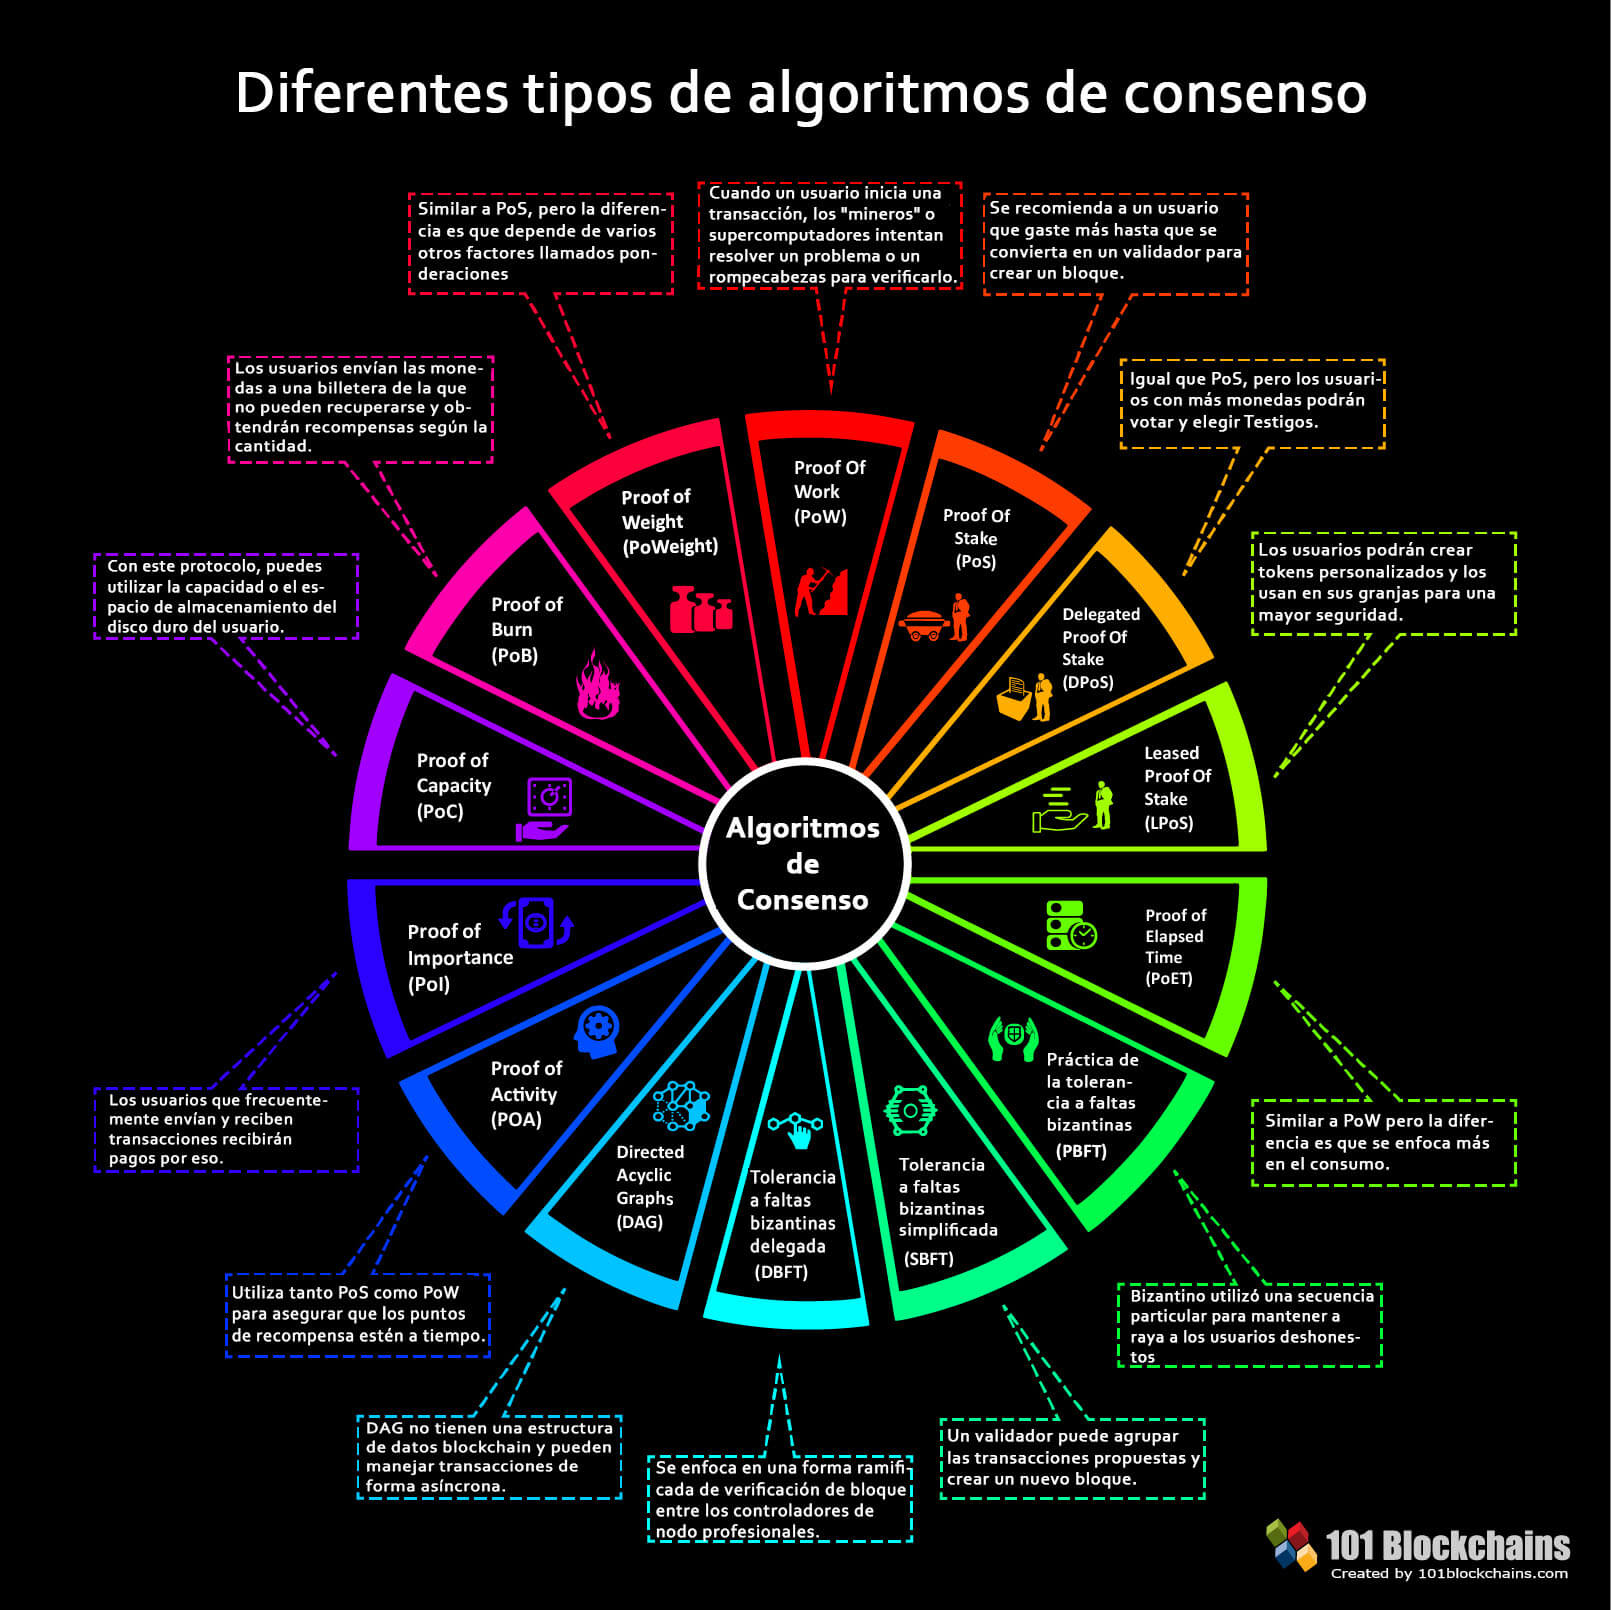
\includegraphics[width=0.8\linewidth]{figs/EstadoArte/Blockchain/algoritmosConsenso.jpeg}
  \caption[Algoritmos de Consenso]{Diferentes tipos de algoritmos de consenso}
  \label{fig:consenso}
\end{figure}

Existen múltiples algoritmos de consenso\ref{fig:consenso}, y estos evolucionan con el paso del tiempo. Los algoritmos de consenso son procesos o protocolos de toma de decisiones, dependiendo del algoritmo hay uno o varios nodos de la red con el poder de tomar la decisión sobre que bloque es el siguiente en añadirse a la red y si ha sido o no alterado. Los objetivos que busca blockchain con los algoritmos de consenso son:

\begin{itemize}
\item Llegar a un acuerdo
\item Cooperación
\item Colaboración
\item Igualdad de derechos
\item Participación
\item Actividad
\end{itemize}

Puesto que hay una gran cantidad de algoritmos trataremos de explicar algunos a continuación\cite{algoConsenso}. Todos los algoritmos buscan el mismo objetivo, solucionar el problema de las \textbf{faltas bizantinas}(BFT)\cite{BFT}. La tolerancia a faltas bizantinas es la resistencia de un sistema informático tolerante a fallas de componentes electrónicos. Si lo llevamos al mundo blockchain, cuando hablamos de fallas nos referimos a nodos de la blockchain defectuosos accidentalmente o provocado. Si una empresa tiene control de 200 nodos, puede tratar de crear transacciones falsas y minar ese bloque con los 200 nodos, el resto de nodos de la red tienen que ser capaces a través del algoritmo de consenso que se utilice de descartar la información de estos 200 nodos.

\subsubsection{Proof of Work (PoW)}

El algoritmo de prueba de trabajo es el primer algoritmo introducido en la red blockchain. Muchas blockchains utilizan este algoritmo para llevar a cabo el consenso y así confirmar todas las transacciones. \\ 

\emph{¿Como funciona?} Cada nodo tiene descargada la red blockchain entera, cuando el nuevo bloque tiene las transacciones necesarias para ser minado, todos los nodos se ponen a buscar el resultado de un \textbf{hash} con la dificultad que tenga el mismo. A más poder de computo, mas posibilidades de encontrar el resultado, validarlo con los otros nodos y añadirlo a la red blockchain, además las redes que usan PoW suelen tener un sistema de premios por lo que cuando un nodo encuentra la solución al problema se le da criptomonedas a cambio. \\

Este sistema tiene dos principales desventajas, la primera es que el poder de cálculo que se necesita es muy grande, y estos últimos años han crecido lo que se conoce como granjas de minado las cuales se llevan el premio la gran mayoría de veces. Esto causa que el sistema empiece a centralizarse, rompiendo con la idea de descentralización que tiene blockchain. El problema es que si alguien logra tener él poder de computo de un 51\% de la red blockchain este puede añadir los bloques que quiera a partir de ese momento pues siempre serán validados por la mayoría de nodos (su 51\% de los nodos). La segunda gran pega va ligada a estas granjas de minado, consumen gran cantidad de energía, en 2020 bitcoin consumió \emph{120 gigawatts} por segundo\cite{bitcoinEnergyUse} lo que a nivel medioambiental tiene un impacto negativo, por lo que PoW no es un algoritmo de consenso que se pueda mantener en el tiempo.

\emph{Ventajas y Desventajas}
\begin{itemize}
\item PROS
  \begin{itemize}
  \item Evita ataques DDoS
  \item Es justo y transparente
  \item Fomenta el interés del público en mantener una red saludable
  \end{itemize}
\item CONS
  \begin{itemize}
  \item La adquisición de equipo para el minado es costosa
  \item La máquina destinada al minado no podrá utilizarse para otra tarea pues se necesita todo el poder de computo en la resolución de los problemas matemáticos (función hash).
  \item La red tiende a centralizarse a causa de las granjas de minado, dándole poder al dueño de la granja y rompiendo la descentralización.
  \item La minería podría desaparecer cuando no haya mas incentivos, en el caso de Bitcoin, cuando se alcance el límite de Bitcoins (21 Millones) los mineros dejarán de recibir premios y se perderá la motivación del minado, no tiene porque desaparecer la red, pero perderá seguidores.
  \end{itemize}
\end{itemize}

\subsubsection{Proof of Stake (PoS)}

El concepto de participación establece que una persona puede minar o validar transacciones en bloque según el número de monedas que posea. Esto significa que cuanta más criptomoneda tengas, más poder de minado se te asigna. \\ 

Se creó como alternativa a PoW, para solventar algunos problemas que tiene (como el de la centralización a causa de las granjas de minado y el gasto energético derivado del poder de computo). PoS solventa este problema atribuyendo la potencia minera a la proporción de monedas que posee un minero. Por lo tanto, en vez de utilizar energía para responder al puzle matemático como hace PoW, aquí el minero se limita a resolver un porcentaje de las transacciones. Si se tiene un 3\% de las criptomonedas disponibles, se puede minar un 3\% de los bloques, en esta ocasión no hay que resolver ningún puzle matemático, simplemente generar un \textbf{hash} con los datos, lo que es una tarea trivial. \\

PoS no es una solución definitiva, pues tiene problemas al igual que PoW. Al igual que antes mencionamos el ataque del 51\% (cuando una empresa o alguien tiene un 51\% de los nodos en su poder). En PoS, si tienes un 51\% de las criptomonedas, tienes un 51\% del poder de decisión sobre la red, pudiendo hacer los cambios que quieras en ella. Este ataque es frecuente en redes pequeñas con pocas criptomonedas en juego, puesto que de lo contrario, lograr tener un 51\% de las monedas supone tener muchísimo dinero. Para controlar estas fraudulencias, se penaliza económicamente a los nodos que tratan de saltarse las reglas (modificar bloques y transacciones), además, un ataque a la blockchain afecta al poder de la moneda y por lo tanto su valor en mercado disminuye, por lo que no compensa tratar de burlar las reglas de la blockchain. Los nodos de las redes que usan PoS, reciben una comisión al minar correctamente su parte del bloque. \\

Redes que utilizan este algoritmo son: Ethereum2.0\cite{Ethereum2.0} y NxT\cite{NxT}.

\subsubsection{Proof of Elapsed Time (PoET)}

La prueba de tiempo transcurrido es un algoritmo que evita la alta utilización de recursos y el alto consumo de energía manteniendo el proceso más eficiente. El algoritmo utiliza un tiempo transcurrido generado aleatoriamente para decidir los derechos de minería y los ganadores de los bloques. Al ejecutar un código de confianza dentro de un entorno seguro, el algoritmo PoET también mejora la transparencia al garantizar que los resultados sean verificables por participantes externos. Este algoritmo se utiliza en redes blockchain permisionadas, por lo que se conoce al dueño de cada nodo. \\

Cada nodo participante en la red debe esperar durante un periodo de tiempo elegido al azar, y el primero en completar el tiempo de espera designado gana el nuevo bloque. Cada nodo de la red blockchain genera un tiempo de espera aleatorio y se pone a dormir durante esa duración especificada. El que se despierta primero, es decir, el que tiene el tiempo de espera más corto, se despierta y añade un nuevo bloque en la cadena de bloques, transmitiendo la información necesaria a toda la red de pares. El mismo proceso se repite para descubrir el siguiente bloque. \\

% -------------------------------------------------- %
\subsection{Smart contracts}

Hasta ahora, hemos hablado de blockchain y criptomonedas, pero las criptomonedas son solo un muy pequeño uso del potencial de blockchain. Los \textbf{Smart Contracts}\cite{etherSmartContract} son un programa que se ejecuta en la red blockchain dando así la capacidad a la red de ser más versátil, al poder ejecutar código (escrito en el smart contract). Básicamente, añade una lógica a la blockchain. \\

Una forma de entender los smart contracts es comparandolos a una máquina de ventas automática. Cuando quieres un snack introduces dinero en la máquina y pones el código del snack, la máquina tiene programada una rutina para verificar que has metido la cantidad adecuada y a cambio devuelve el snack seleccionado. Ese programa interno que tiene la máquina, es el equivalente a un \textbf{smart contract}. \\


Al estar programados en la red blockchain, no pueden ser modificados sin que todos los nodos se enteren. De hecho, cuando se quiere actualizar un smart contract, no se actualiza el existente en la red, sino que se realiza una nueva transacción la cual ha de ser validada por el resto de nodos. Los smart contracts permiten que se realicen transacciones y acuerdos de confianza entre partes dispares y anónimas sin necesidad de una autoridad central, un sistema legal o un mecanismo de aplicación externo. No se puede evadir o sortear al smart contract, cuando realizas una llamada a una de sus funciones no hay forma humana de lograr burlarlo, la rutina se ejecutará siempre sin fallos. El equivalente se puede ver como tener a un notario robótico el cual nunca comete errores.  \\

\label{sec:smartContract}
\index{SmartContract}

% \begin{lstlisting}[language=Java,float=ht,caption={[Smart Contract]Ejemplo de código fuente de un smart contract escrito en Solidity},label=lst:java]
% pragma solidity 0.6.11;
% 
% contract VendingMachine {
%   // Declare state variables of the contract
%   address public owner;
%   mapping (address => uint) public cupcakeBalances;
% 
%   // When 'VendingMachine' contract is deployed:
%   // 1. set the deploying address as the owner of the contract
%   // 2. set the deployed smart contract's cupcake balance to 100
%   constructor() public {
%     owner = msg.sender;
%     cupcakeBalances[address(this)] = 100;
%   }
% 
%   // Allow the owner to increase the smart contract's cupcake balance
%   function refill(uint amount) public {
%     require(msg.sender == owner, "Only the owner can refill.");
%     cupcakeBalances[address(this)] += amount;
%   }
% 
%   // Allow anyone to purchase cupcakes
%   function purchase(uint amount) public payable {
%     require(msg.value >= amount * 1 ether, "You must pay at least 1 ETH per cupcake");
%     require(cupcakeBalances[address(this)] >= amount, "Not enough cupcakes in stock to complete this purchase");
%     cupcakeBalances[address(this)] -= amount;
%     cupcakeBalances[msg.sender] += amount;
%   }
% }
% \end{lstlisting}

\begin{figure}[h!]
  \centering
  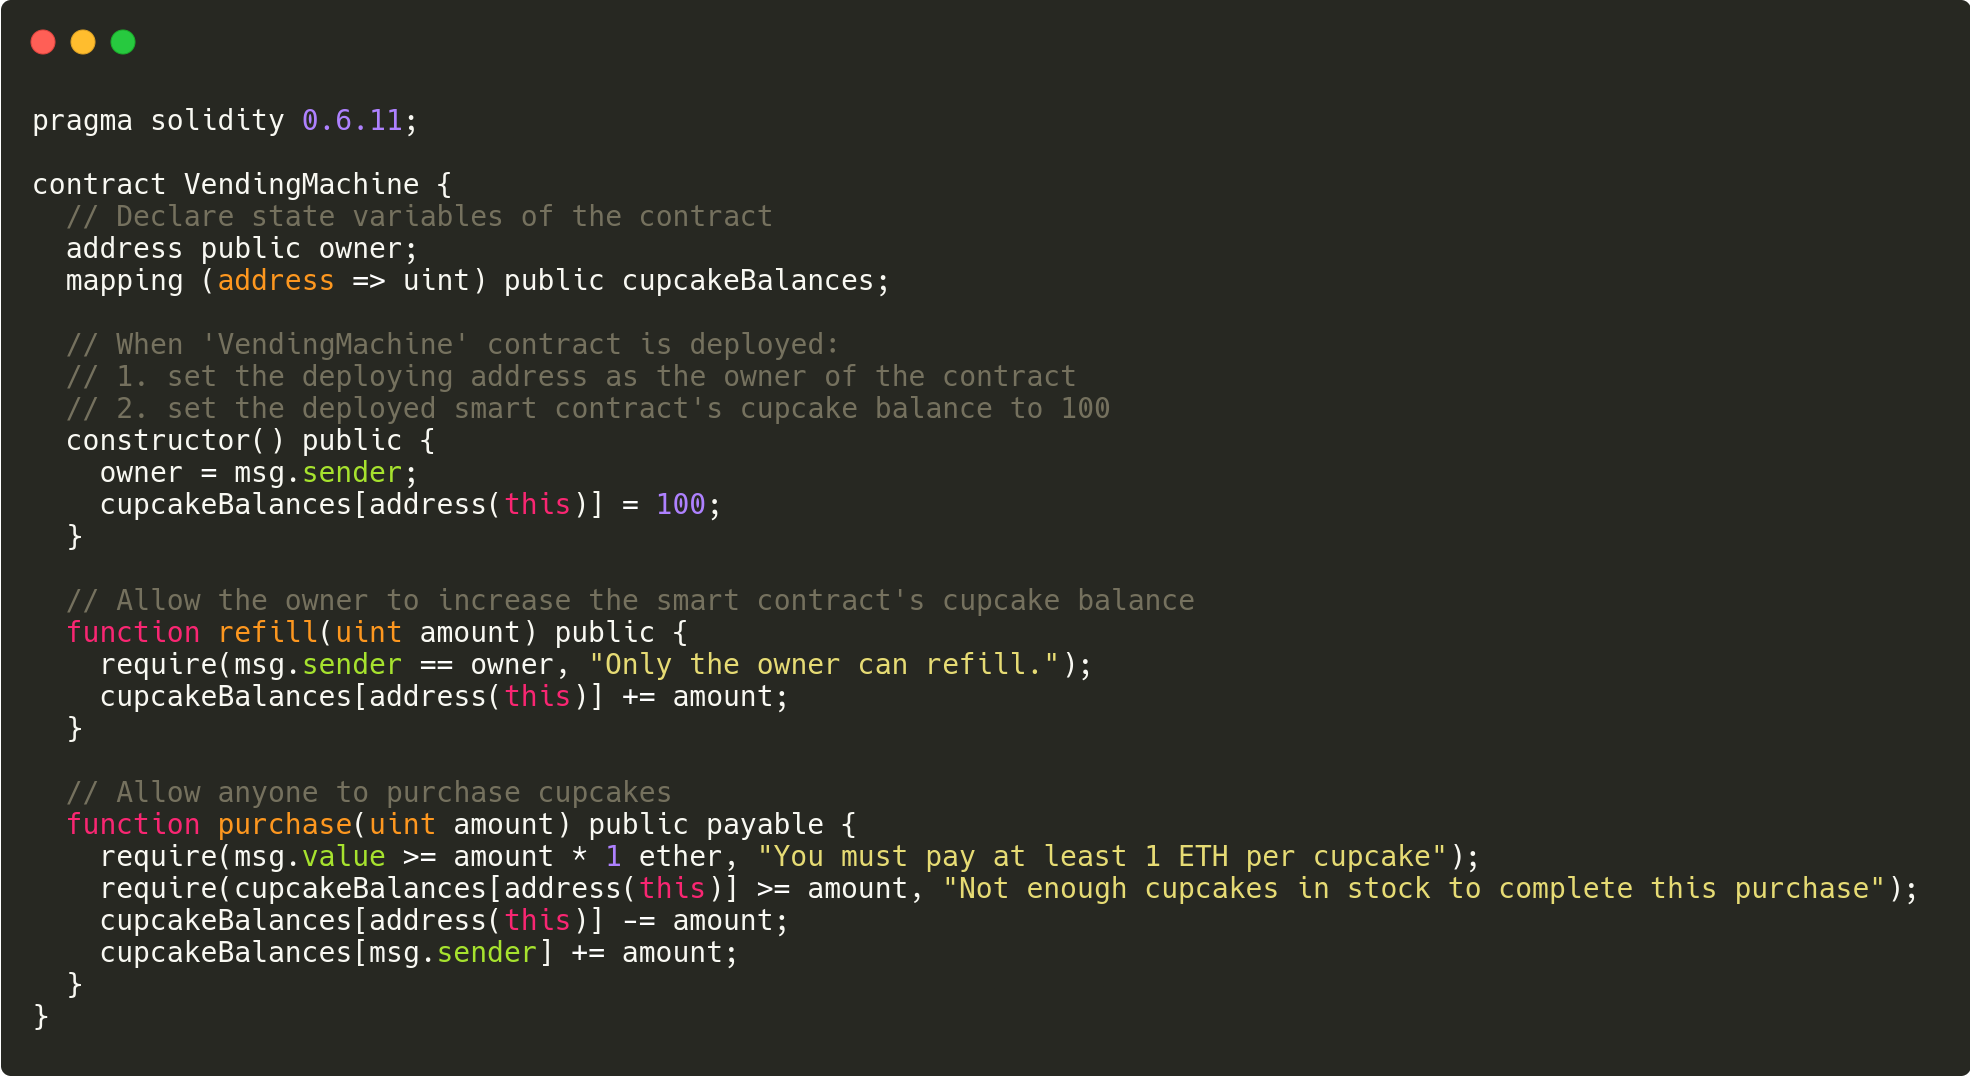
\includegraphics[width=0.8\linewidth]{figs/EstadoArte/Blockchain/SmartContractEjemplo}
  \caption[Máquina de ventas en solidity]{Máquina de ventas en solidity}
  \label{fig:smartContract}
\end{figure}


Los smart contracts pueden ser escritos en múltiples lenguajes de programación dependiendo de la red blockchain que se vaya a utilizar. Algunos ejemplos son:
\begin{itemize}
\item EOS Blockchain -> \verb|C++|
\item Ethereum -> \verb|Solidity|\ref{fig:smartContract}
\item NEO Blockchain -> \verb|JavaScript, Java|
\item Hyperldger -> \verb|Golang|
\item Cardano -> \verb|Haskell|
\end{itemize}

La primera red blockchain en explotar el potencial de los smart contracts fue \textbf{ethereum} y puesto que es la red blockchain sobre la cual se apoyará la aplicación Android que voy a desarrollar en este TFG, procederé a analizarla.

% -------------------------------------------------- %
\subsection{Usos en el presente de Blockchain}
En el presente están en desarrollo múltiples aplicaciones basadas en Blockchain:

\begin{itemize}
\item Criptomonedas: \textit{Bitcoin, Ethereum, Tether, Cardano, XRP, Litecoin, ChainLink, Dogecoin, TRON, VeChain, Monero, BitTorrent, Kusama, Neo, Dai, NEM, Dash, Maker}\dots \cite{listaCripto}.
\item Firma digital y verificación de la identidad: Startups como \textit{Civic} o \textit{Niuron}\cite{civic, niuron} buscan implementar firmas digitales para notarios y bancos y check-in telemáticos en hoteles y pisos turísticos.
\item Trazabilidad alimentaria: Empresas como carrefour implementan trazabilidad de sus alimentos con la ayuda de IBM \cite{carrefour}
\item Turismo y Hoteles: La empresa \textit{TUI Group} cuenta con más de 300 hoteles y esta moviendo sus activos inmobiliarios y procesos internos a una blockchain \cite{tuig}.
\item Votaciones y elecciones: El \textit{Banco Santander} utilizó en 2018 con éxito una red blockchain para votar a su Junta General de Accionistas\cite{santanderVotacion}
\end{itemize}

Y mucho más \cite{appCripto}.

% -------------------------------------------------- %
\section{Ethereum}

\begin{figure}[h!]
  \centering
  
\includegraphics[width=0.2\linewidth]{figs/EstadoArte/Ethereum/ethereumLOGO}
  \caption[Ethereum]{Logo de ethereum}
  \label{fig:ethereum}
\end{figure}

\textit{Ethereum\ref{fig:ethereum} es una plataforma global de código abierto para aplicaciones descentralizadas, permite escribir código que controla el valor digital, funciona tal como se programó y al que puede accederse desde cualquier parte del mundo. Ethereum es un acceso abierto al dinero digital y a los servicios de información para todos, sin importar su origen o ubicación. Es una tecnología creada por la comunidad tras la criptomoneda ether (ETH) y miles de aplicaciones que puedes usar hoy.}

% -------------------------------------------------- %
\subsection{Ether (ETH)}
La moneda que utiliza la red de Ethereum es el \textbf{ether}, se utiliza para recompensar a los mineros que aseguran las transacciones. \emph{Ethereum1.0} utiliza el algoritmo \textit{PoW} y \emph{Ethereum2.0} utiliza \textit{PoS}\cite{Ethereum2.0}. Los ethers se utilizan como almacén de valor, prestamos de garantía, medio de intercambio, unidad de cuenta en mercados digitales \dots \\

Cada transacción en ethereum lleva asociado un coste conocido como \textbf{gas}. El gas es la unidad que se utiliza para ver el coste de computo que tiene la transacción, para poder remunerar adecuadamente al minero. La unidad de gas se mide en \textbf{Gwei}\cite{Gwei} si por ejemplo queremos enviar una cantidad \verb|X| de ether a otra persona esta transacción tiene un coste de \verb|21.000|Gwei lo que es equivalente a \verb|0,000021 ETH| (1ETH = $10^9$Gwei)

% -------------------------------------------------- %
\subsection{Carteras}

Las carteras de ethereum son aplicaciones que permiten a los usuarios interactuar con sus cuentas de ethereum. Se las puede ver como una aplicación bancaria. Tu cartera te permite leer tu saldo, enviar transacciones y conectarte a aplicaciones. Se necesita una cartera para enviar fondos y gestionar tu ETH. Pero es únicamente una herramienta para gestionar tu cuenta, puedes cambiar de cartera sin problema pues no es quien custodia tus fondos, eres tú quien los custodia en todo momento. \\

La cartera tiene asociado un \textbf{address}, un address es el identificador que tiene tu cuenta en la red de ethereum, es único para ti. Si alguien quiere enviarte dinero lo hará desde su address a tú address, si quieres hacer una llamada a un Smart Contract, al smart contract le llegará como información tú address. \\

A grandes rasgos nos quedan estos tres términos importantes:
\begin{itemize}
\item \textbf{Cuenta} de ethereum.
\item \textbf{Address} de la cuenta.
\item \textbf{Cartera} para gestionar la cuenta.
\end{itemize}

% -------------------------------------------------- %
\subsection{Ethereum Smart Contract}

Los smart contracts de ethereum están escritos en \textbf{Solidity}\cite{SolidityDocs}\ref{fig:soliditySmartContractEntero} o \textbf{Vyper}\cite{VyperDocs}, sus logos pueden verse en \ref{fig:programas}. Cualquier persona es libre de programar un smart contract y desplegarlo en la red de ethereum, los smart contracts son una transacción más y tienen su propio address. Permitiendo que cualquier persona haga llamadas al smart contract. Desplegar un smart contract cuesta \emph{gas} al igual que cualquier transacción, sin embargo es bastante más caro. 

\begin{figure}[h!]
  \centering
  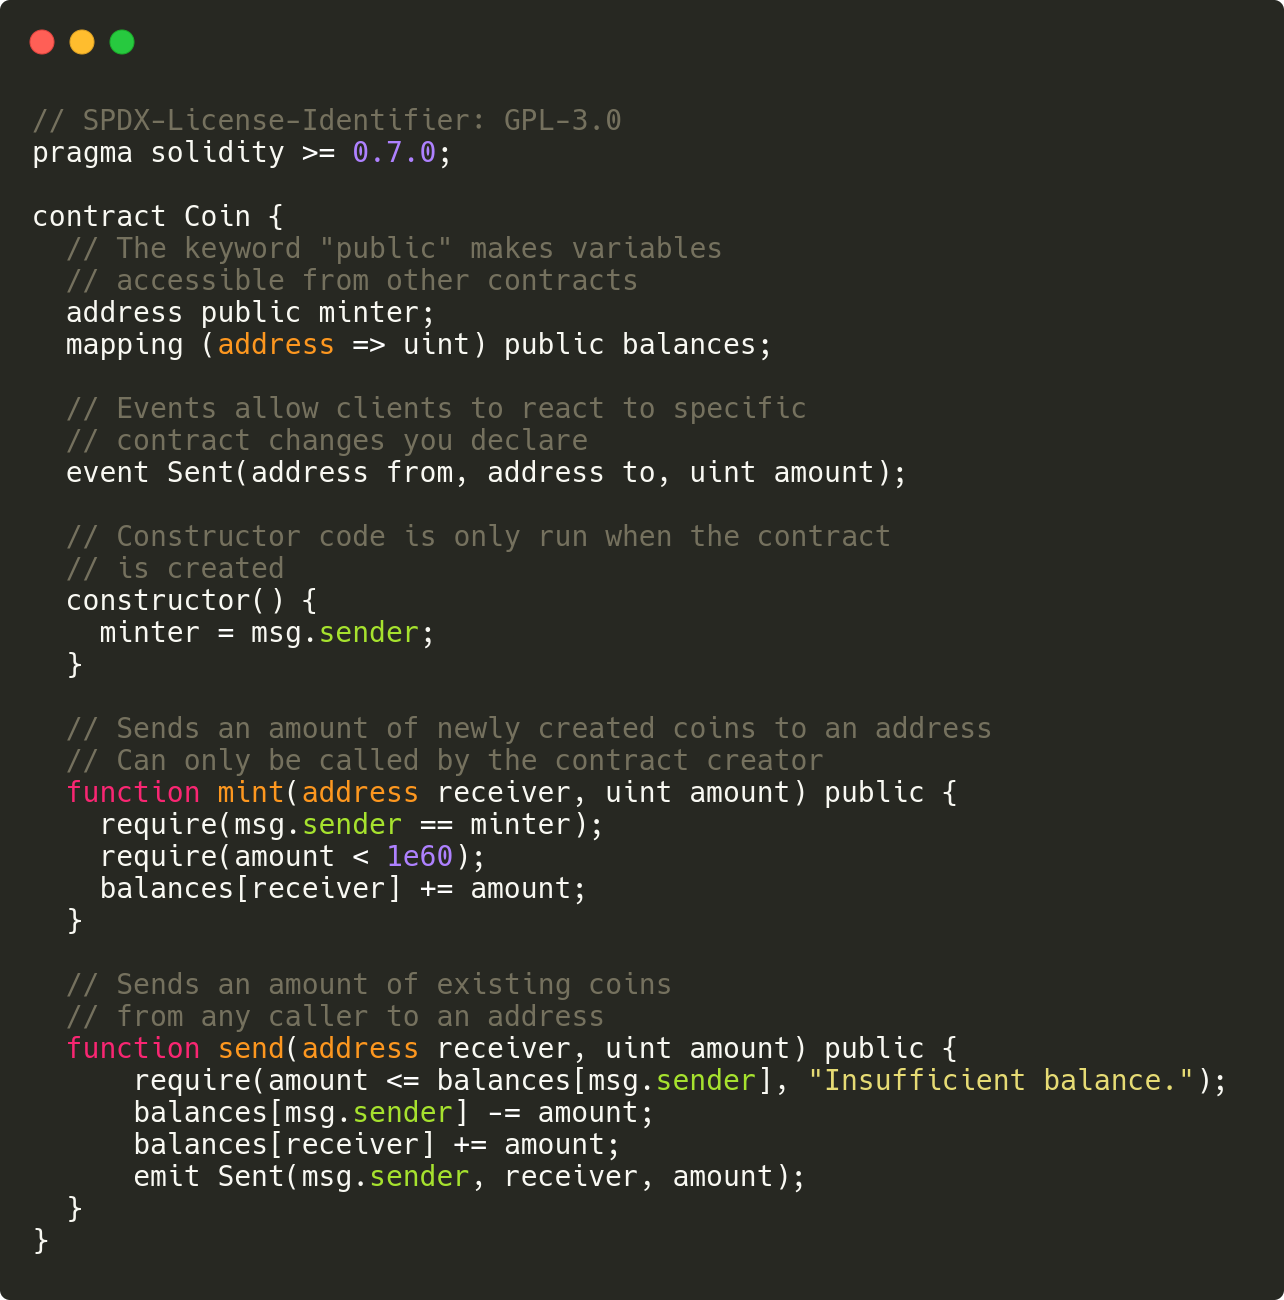
\includegraphics[width=0.7\linewidth]{figs/EstadoArte/Ethereum/SmartContract}
  \caption[Código ejemplo de un smart contract]{Código ejemplo de un smart contract}
  \label{fig:soliditySmartContractEntero}
\end{figure}

\begin{figure}[hbt]
	\centering
	\begin{subfigure}[b]{0.4\linewidth}
		\centering
		
\includegraphics[width=0.5\linewidth]{figs/EstadoArte/Ethereum/solidityLOGO}
		\caption{Logo de Solidity}\label{fig:solProgram}
	\end{subfigure} 
	\begin{subfigure}[b]{0.4\linewidth}
		\centering
		
\includegraphics[width=0.6\linewidth]{figs/EstadoArte/Ethereum/vyperLOGO}
		\caption{Logo de Vyper}\label{fig:vyperProgram}
	\end{subfigure} 
	\caption[Lenguajes de Smart Contract]{Lenguajes de smart contract para ethereum.}
	\label{fig:programas}
\end{figure}

% \begin{lstlisting}[language=Java,float=ht,caption={[Solidity Contract]Ejemplo de código fuente de un smart contract escrito en Solidity},label=lst:java]
% // SPDX-License-Identifier: GPL-3.0
% pragma solidity >= 0.7.0;
% 
% contract Coin {
%   // The keyword "public" makes variables
%   // accessible from other contracts
%   address public minter;
%   mapping (address => uint) public balances;
% 
%   // Events allow clients to react to specific
%   // contract changes you declare
%   event Sent(address from, address to, uint amount);
% 
%   // Constructor code is only run when the contract
%   // is created
%   constructor() {
%     minter = msg.sender;
%   }
% 
%   // Sends an amount of newly created coins to an address
%   // Can only be called by the contract creator
%   function mint(address receiver, uint amount) public {
%     require(msg.sender == minter);
%     require(amount < 1e60);
%     balances[receiver] += amount;
%   }
% 
%   // Sends an amount of existing coins
%   // from any caller to an address
%   function send(address receiver, uint amount) public {
%       require(amount <= balances[msg.sender], "Insufficient balance.");
%       balances[msg.sender] -= amount;
%       balances[receiver] += amount;
%       emit Sent(msg.sender, receiver, amount);
%   }
% }
% \end{lstlisting}

% -------------------------------------------------- %
\subsection{Funcionamiento básico de Ethereum}

Para entender el funcionamiento básico de Ethereum, vamos a exponerlo por niveles como lo hacen en la documentación oficial\cite{etherStack}. 

% -------------------------------------------------- %
\subsection{Nivel 1: Máquina Virtual de Ethereum} 

La \textbf{EVM}\ref{fig:evm} es el entorno de ejecución de los smart contract. Esta, gestiona todo el procesamiento de transacciones en la red, creando un nivel de abstracción entre el código que se ejecuta y la máquina que lo hace. La EVM es \emph{Turing-Completa} con 140 instrucciones únicas que la permiten ejecutar casi cualquier cosa. 

\begin{figure}[h!]
  \centering
  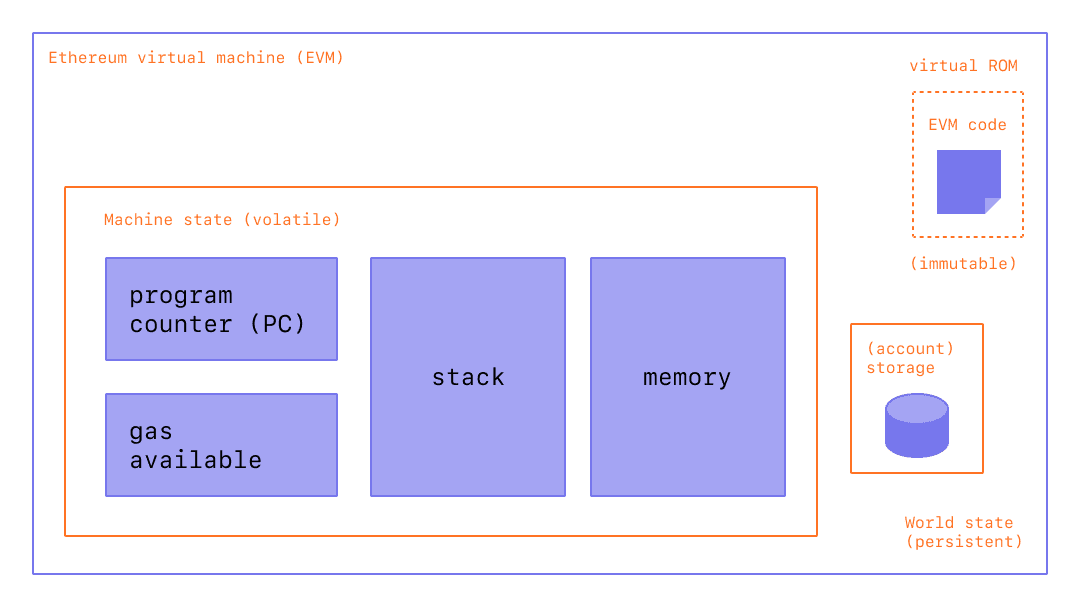
\includegraphics[width=0.8\linewidth]{figs/EstadoArte/Ethereum/evm}
  \caption[Diagrama EVM]{Diagrama de la máquina virtual de ethereum}
  \label{fig:evm}
\end{figure}

% -------------------------------------------------- %
\subsection{Nivel 2: Smart Contract} 

Programas que se ejecutan en la red de ethereum. 

% -------------------------------------------------- %
\subsection{Nivel 3: Nodos de Ethereum}

Para que una app pueda interactuar con la red, necesita conectarse a un nodo de ethereum\ref{fig:etherNodo}. Los nodos son ordenadores que ejecutan el \emph{software} cliente de ethereum, manteniendo el registro de bloques y validando las transacciones. Almacenan colectivamente el estado de la blockchain y llegan a un consenso sobre las transacciones para hacer crecer el número de bloques. Al conectar la app con un nodo, la app puede leer datos de la red, enviar nuevas transacciones\dots

\begin{figure}[h!]
  \centering
  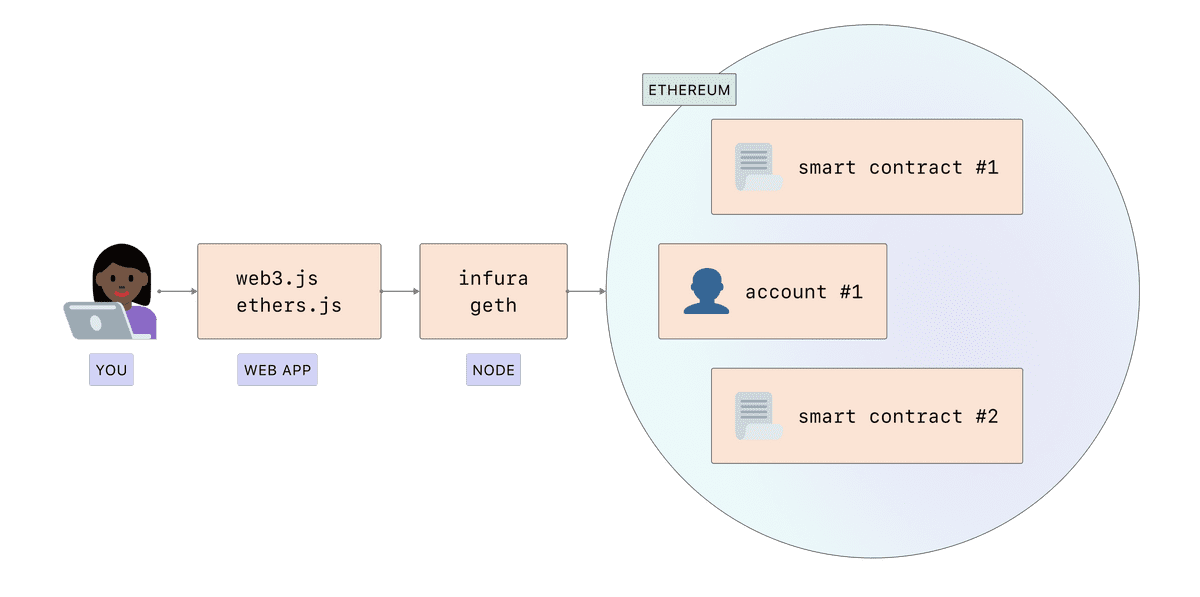
\includegraphics[width=0.8\linewidth]{figs/EstadoArte/Ethereum/ethereumNodo}
  \caption[Nodos vista genérica]{Nodo y vista genérica de aplicaciones.}
  \label{fig:etherNodo}
\end{figure}

% -------------------------------------------------- %
\subsection{Nivel 4: API para el cliente de ethereum}

Las APIs permiten a los desarrolladores abstraer parte de la dificultad de interactuar directamente con los nodos de ethereum. Además proporcionan herramientas como para convertir datos de ETh a Gwei\dots Existen APIs en \verb|JavaScript, Java, Python| por ejemplo, una de las más conocidas es la librería \textbf{Web3}\cite{web3} la cual evita al programador tener que implementar la comunicación con los nodos. 

% -------------------------------------------------- %
\subsection{Nivel 5: Aplicaciones para usuario}

En el nivel superior están las apps orientadas al usuario. Principalmente son aplicaciones web y móvil. Las aplicaciones se construyen de la manera tradicional, y utilizan las APIs necesarias para comunicarse con la red y/o smart contracts. Las aplicaciones distribuidas o aplicaciones que funcionan gracias a una red blockchain, se las conoce como \textbf{Dapps}, básicamente son como una aplicación tradicional, pero ejecutadas en una red punto a punto \textit{peer-to-peer (P2P)} como blockchain.

% -------------------------------------------------- %
% -------------------------------------------------- %
\section{Aplicaciones móvil que usan Blockchain}

Ahora que entendemos que es Blockchain, visto múltiples ejemplos de redes, visto múltiples aplicaciones de la red Blockchain, y hemos indagado más sobre Ethereum y lo Smart Contract, vamos a pasar a ver los proyectos actuales que utilizan aplicaciones móvil y blockchain. Puesto que el objetivo de este \textbf{TFG} es el desarrollo de una aplicación Android que comunique con una blockchain para luego sacar esa funcionalidad en un SDK.

% -------------------------------------------------- %
\subsection{GUTS Tickets}

Esta aplicación móvil usa blockchain para emitir entradas honestas que ponen fin a los vergonzosos precios del mercado de la ``reventa'' y al fraude en las entradas. \emph{GUTS}\ref{fig:Logos} es el primer sistema de ventas de entradas que hace uso del \textbf{Protocolo de Entrada Garantizada} {\small (\textit{Guaranteed Entrance Protocol (GET)})}\cite{GET}\ref{fig:Logos}. Este protocolo permite crear entradas inteligentes y seguras permitiendo el seguimiento de las mismas así como el control de su precio original y secundario (reventa). 

\begin{figure}[hbt]
	\centering
	\begin{subfigure}[b]{0.4\linewidth}
		\centering
		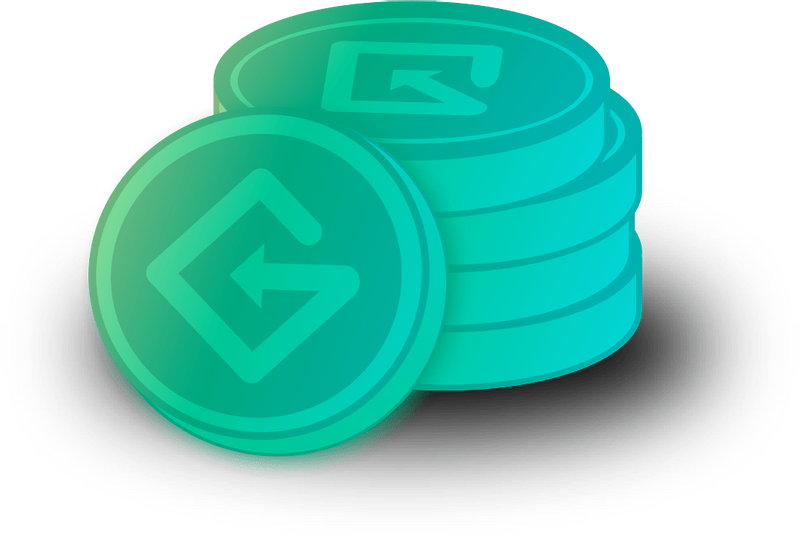
\includegraphics[width=0.8\linewidth]{figs/EstadoArte/Apps/getTOKEN.png}
		\caption{Logo del token de GET}\label{fig:getTOKEN}
	\end{subfigure} 
	\begin{subfigure}[b]{0.4\linewidth}
		\centering
		
\includegraphics[width=0.6\linewidth]{figs/EstadoArte/Apps/gutsLOGO.png}
		\caption{Logo de la aplicación Guts}\label{fig:gutsLOGO}
	\end{subfigure} 
	\caption[Logos de Guts y GET]{Logos}
	\label{fig:Logos}
\end{figure}

\subsubsection{Protocolo GET}

El protocolo GET ofrece una solución de emisión de billetes inteligentes basadas en blockchain que puede ser utilizada por todos los que necesitan emitir billetes de forma transparente, segura y honesta. Evitando fraudes, y vergonzosas subidas del precio de las entradas en el mercado de la reventa. La funcionalidad de registro de entradas de GET funciona con un SmartContract escrito en solidity, su código fuente es de código abierto \cite{srcGET}. La blockchain que utiliza para apoyarse es la de \emph{Ethereum}, y disponen de \textbf{Token} propio para realizar las transacciones\cite{tokGET}. GET guarda un historial para cada tickets utilizando \textbf{IPFS}\cite{IPFS} que luego guarda en la red blockchain con el smart contract, \textit{IPFS, es un sistema distribuido que permite guardar y recuperar archivos, webs, aplicaciones\dots y pretende superar a HTTP para construir una web mejor para todos}.

% -------------------------------------------------- %
\subsection{LifeID}

Esta aplicación esta construyendo una plataforma de identidad digital segura y basada en blockchain. Con una sencilla aplicación móvil te ofrece el control sobre la gestión de tú identidad digital. Permite iniciar sesión en cualquier sitio, entrar en cualquier edificio en el que se requiera de autenticación o participar en transacciones basadas en la identidad (como puede ser en un sistema de votación) todo con la tranquilidad, fiabilidad y control que da la blockchain. \\ 

Para ello utiliza la red blockchain de \textbf{ArcBlock}\cite{webArc,alianzaArc}. ArcBlock es una plataforma para desarrollar aplicaciones en blockchains o \textbf{DApps}\cite{dapps}. 

\subsection{Voatz}

Voatz\ref{fig:Voatz} es una plataforma electoral móvil que permite a los ciudadanos votar sin tener que acudir a su colegio electoral o presentar una papeleta por correo. Voatz aprovecha las características de seguridad integradas en las últimas versiones de la tecnología de los teléfonos como es la biometría. Y también aprovecha la seguridad, transparencia e inmutabilidad de la red blockchain para garantizar la seguridad de cada voto. Desde el 2016 han emitido más de 110000 votos en mas de 67 elecciones. 

\begin{figure}[h!]
  \centering
  
\includegraphics[width=0.6\linewidth]{figs/EstadoArte/Apps/voatz}
  \caption[Nodos vista genérica]{Logo de la aplicación Voatz.}
  \label{fig:Voatz}
\end{figure}



% ###########################################
% ###########################################
\section{Android}

Android\cite{android} es un sistema operativo móvil basado en el \emph{Linux Kernel}. Fue diseñado para dispositivos móvil inteligentes, con pantallas táctiles, disponible para tablets, relojes inteligentes, incluso hay versiones de Android para el software de automóviles\cite{androidAuto}. Android es el sistema operativo móvil más utilizado del mundo, con una cuota de mercado superior al 90\% en 2018. Su código fuente es abierto y libre para que cualquiera pueda consultarlo o contribuir a él. Actualmente se encuentra en la versión \textbf{11} internamente conocido como ``Red Velvet Cake'' pero son pocos los móviles con opción a ella, a la hora de desarrollar una aplicación para dispositivos Android, lo ideal es elegir la versión \textbf{6} también conocido como ``Oreo'' la cual puede ejecutar una gran mayoría. 

% --------------------------------------------------
\subsection{Conceptos Básicos de Android}

A la hora de programar aplicaciones en Android, lo ideal es trabajar en paralelo con la documentación para desarrolladores\cite{androidDocs}. En ella se detalla el completo funcionamiento y diferentes APIs disponibles para programar las aplicaciones. Para este apartado resumo algunos de los conceptos de la guía, siendo una gran recomendación si se quiere profundizar más ir directamente a la guía. \\

Las aplicaciones de Android se pueden escribir con \textbf{Kotlin, Java y C++}\cite{kotlin,java,c++}. Una vez escrito el código fuente, las herramientas de Android SDK compilan el código generando un paquete o APK, el cual incluye todos los contenidos de la aplicación Android y permite ser ejecutado en un dispositivo móvil (el dispositivo requerirá de la versión Android mínima para poder ejecutar.). \\

Cada aplicación de Android reside en su propia ``zona virtual'', un conjunto de factores permiten tener aisladas las aplicaciones Android del resto del móvil. Entre otras, puesto que Android reside en un sistema Linux, el cual es multiusuario, cada aplicación en el móvil es un usuario el cual puede acceder solo a sus archivos y documentos teniendo sus propios permisos como usuario dentro del dispositivo y creando lo grupos que necesite. Cada proceso que se ejecuta tiene su propia máquina virtual, ejecutándose el código de forma independiente al resto de aplicaciones. Es el sistema operativo el que se encarga de mantener los distintos procesos, así como arrancar procesos que sean requeridos por la aplicación. \\

Un ejemplo, si desde la aplicación de galería queremos compartir una foto por Whatsapp, la aplicación ``galería'' le pedirá al SO que ejecute una actividad de ``Whatsapp'' y será el SO quien se encargue de decidir si tiene permiso para eso o no, o si tiene recursos para ejecutarlo o no. En ningún momento la aplicación ``galería'' tiene libertad para ejecutar otros procesos. \\

De forma predeterminada las aplicaciones solo tiene derecho de usar sus propios archivos, pero puede pedir permiso al sistema operativo para guardar información en el dispositivo, en el caso de mi aplicación Android por ejemplo, el registro de claves para acceder a la blockchain se guardan de forma local en el dispositivo. También, la aplicaciones pueden pedir permiso para utilizar cámara, conexión bluetooth\dots \\

Por último, algo muy importante a tener en cuenta al programar aplicaciones Android es que no puedes hacer operaciones pesadas en el hilo de ejecución principal. Todas las ejecuciones pesadas deben hacerse en otro hilo y con un callback recuperar la información si es necesario. Por ejemplo, al hacer llamadas a una API estas llamadas deben hacerse en otro hilo de ejecución diferente. Android no permite que bloquees la interfaz de usuario con operaciones pesadas (como una llamada a una API).

\subsubsection{Componentes de la aplicación}

Las aplicaciones Android tienen:
\begin{itemize}
    \item Actividades
    \item Servicios
    \item Receptores de emisiones
    \item Proveedores de contenido
\end{itemize}
\vspace{0.5cm}
\textbf{Actividades} \\
Las \textbf{Actividades} son el punto de entrada de interacción con el usuario. Se representan como una pantalla con una interfaz de usuario. Por ejemplo, Whatsapp tiene una actividad que es la pantalla en la que todos los grupos y gente con la que hablas, y al entrar en un grupo, Whatsapp ejecuta una actividad diferente. Las actividades trabajan juntas pero son independientes entre si, brindando la posibilidad de llamar a una actividad concreta desde otra aplicación. Si quieres compartir una foto con un grupo en Whatsapp, desde la app de galería seleccionas la foto y llamas a la actividad de Whatsapp del grupo de amigos concreto con quienes quieres compartir la foto. Las actividades permiten:

\begin{itemize}
\item Realizar un seguimiento de la pantalla que esta viendo el usuario.
\item Permitir regresar a actividades anteriores (actividades detenidas) a las que puede volver el usuario si lo desea, priorizando entonces algunos procesos mas que otros.
\item Permitir finalizar procesos, volviendo a la actividad anterior.
\item Permitir ser llamadas desde otras aplicaciones (como el ejemplo de compartir una imagen)
\end{itemize}

\vspace{0.5cm}
\textbf{Servicios} \\
Los \textbf{Servicios} son un punto de entrada general que permite mantener en ejecución una aplicación en segundo plano y no proporcionan una interfaz de usuario. Un servicio puede reproducir música, sincronizar datos\dots Además los servicios pueden dividirse en 2, \textbf{servicios iniciados} y \textbf{servicios enlazados}. Los iniciados son servicios que inicia el usuario como reproducir música dejando luego el proceso en segundo plano. Y un servicio enlazado sería cuando una aplicación hace uso de otra para alguna tarea. Esta segunda aplicación que esta siendo usada, se ejecuta en segundo plano como servicio enlazado. \\

\textbf{Receptores de emisiones} \\
Los \textbf{receptores} permiten que el sistema entregue eventos a una aplicación fuera del flujo habitual. El sistema puede entregar emisión de aplicaciones que no están en ejecución. Por ejemplo, una aplicación programa una alarma a una hora determinada, aunque la aplicación no este en ejecución, la alarma sonará a la hora establecida. Muchas de las emisiones, vienen del propio sistema. Por ejemplo, pantalla apagada, batería baja, captura de pantalla\dots Los receptores de emisión no disponen de interfaz de usuario, pero a través de la API de Android pueden mostrar mensajes en la barra de tareas. \\

\textbf{Proveedores de contenido} \\
Los \textbf{proveedores de contenido} administran conjuntos compartidos de datos de la aplicación que pueden ser almacenados en el sistema de archivos, en una BDD o en la web. A través del proveedor de contenido, otras aplicaciones pueden acceder a esos datos (siempre que tengan permiso). Por ejemplo, la aplicación de contactos del móvil, tiene un proveedor de contenido, lo que permite a otras aplicaciones pedir acceso a la agenda de datos (siendo el usuario el que acepta que la aplicación acceda a los contactos). También son útiles para leer y escribir datos privados que no quieras compartir con otras aplicaciones.

\subsubsection{Activación de componentes}

Un aspecto exclusivo de Android es que cualquier aplicación puede iniciar un componente de otra aplicación. Si quieres que el usuario tome una foto, no hace falta desarrollar la comunicación con el hardware de la cámara, sino que simplemente puedes llamar a la aplicación de la cámara la cual te devolverá la foto que el usuario tome. Por ejemplo, si inicias la actividad de la cámara, la actividad se ejecuta en el proceso de la cámara no en tú aplicación. Por lo tanto, a diferencia de lo que sucede en las aplicaciones de otros sistemas, aquí no existe un método principal o \verb|main()|. Android no tiene un único punto de entrada. \\

De los cuatro tipos de componente, actividades, servicios y receptores se activan mediante un mensaje asíncrono denominado \verb |intent|, estos vinculan componentes entre sí durante el tiempo de ejecución. Son algo así como mensajeros. Sin embargo, los proveedores de contenido se activan con solicitudes de un \verb|ContentResolver|. Además, existen para cada componente métodos independientes para activarlos según el objetivo que se busque.
\subsubsection{El archivo de manifiesto}

Para que Android pueda iniciar un componente, debe reconocer la existencia de ese componente leyendo el archivo de manifiesto de la aplicación, \verb|AndroidManifest.xml|. El manifiesto puede hacer lo siguiente:
\begin{enumerate}
    \item Declarar los componentes de la aplicación
    \item Identificar los permisos de usuario que requiere la aplicación (acceso a internet, o acceso a los contactos)
    \item Declarar características hardware y software así como nivel de API mínimo.
    \item Declarar APIs a las que la aplicación necesita estar vinculado (como la biblioteca de google maps)
\end{enumerate}

\subsubsection{Recursos de la aplicación}

Las aplicaciones Android se componen de mucho más que solo código. Disponen de imágenes, vídeos, fuentes, audios y otros elementos como las interfaces de usuario en XML. Los recursos facilitan la actualización de las características de la aplicación para permitir el cambio de idioma, de fuente, de tamaño según el dispositivo\dots \\

Por cada recurso, el SDK define un ID con número entero único para poder hacerle referencia. Estos IDs se utilizan en el código, por ejemplo, para añadir una imagen puedes hacer referencia al ID de la imagen asignado por el SDK. Una de las ventajas de utilizar los recursos, es facilitar la traducción de la aplicación a otros idiomas, también puedes mostrar parte de la interfaz de usuario si el usuario tiene una suscripción concreta u otra. En el caso de mi aplicación móvil, utilizo esto para mostrar una aplicación diferente  a los alumnos y profesores.



% --------------------------------------------------
\section{Desarrollo de Microservicio Externo}

Para poder desarrollar la aplicación móvil y el SDK de este TFG, se ha desarrollado previamente una API de microservicios la que centralizar las llamadas a una base de datos y a una red blockchain, básicamente es para agilizar las llamadas y tratamiento de datos por parte del dispositivo móvil, así como minimizar la cantidad de código, tamaño de la aplicación móvil, dependencias del proyecto\dots La API de microservicios con la que se comunica la aplicación móvil se ha desarrollado utilizando \textbf{NodeJS} y ha sido documentada utilizando \textbf{Swagger} \ref{fig:swaggerQuerys}, \ref{fig:swaggerUsuario}. \\

\begin{figure}[h!]
  \centering
  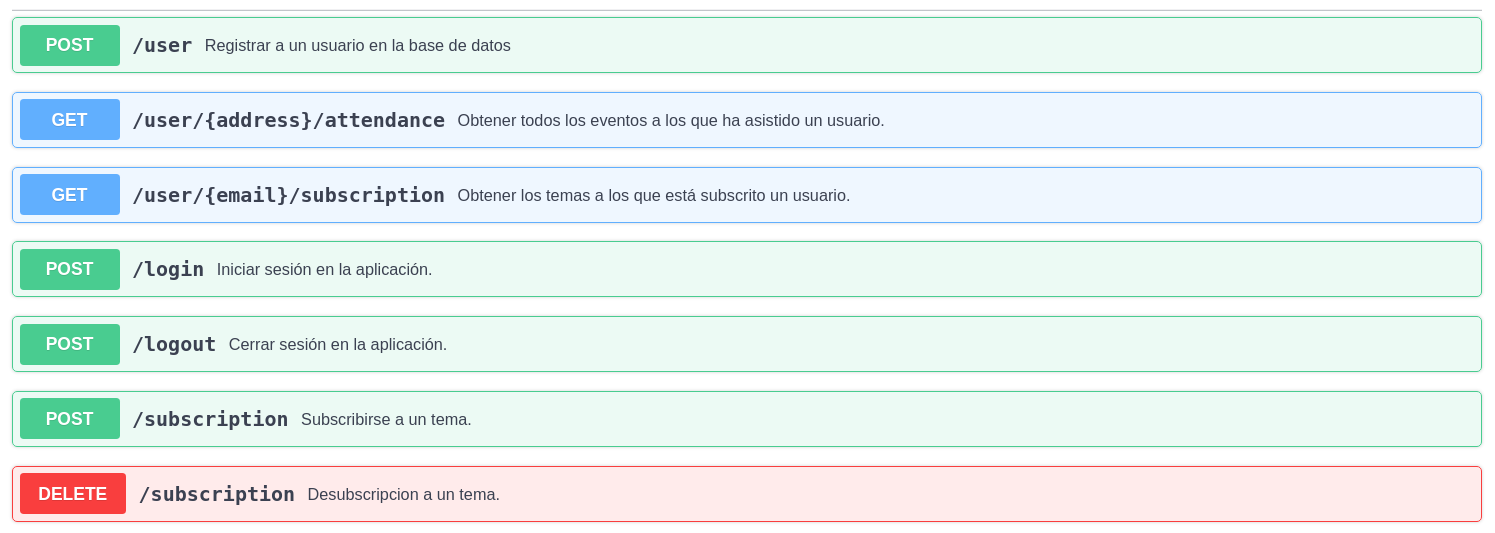
\includegraphics[width=1\linewidth]{figs/Desarrollo/Swagger}
  \caption[Swagger]{Fragmento de documentación en Swagger del Proyecto}
  \label{fig:swaggerQuerys}
\end{figure}

\begin{figure}[h!]
  \centering
  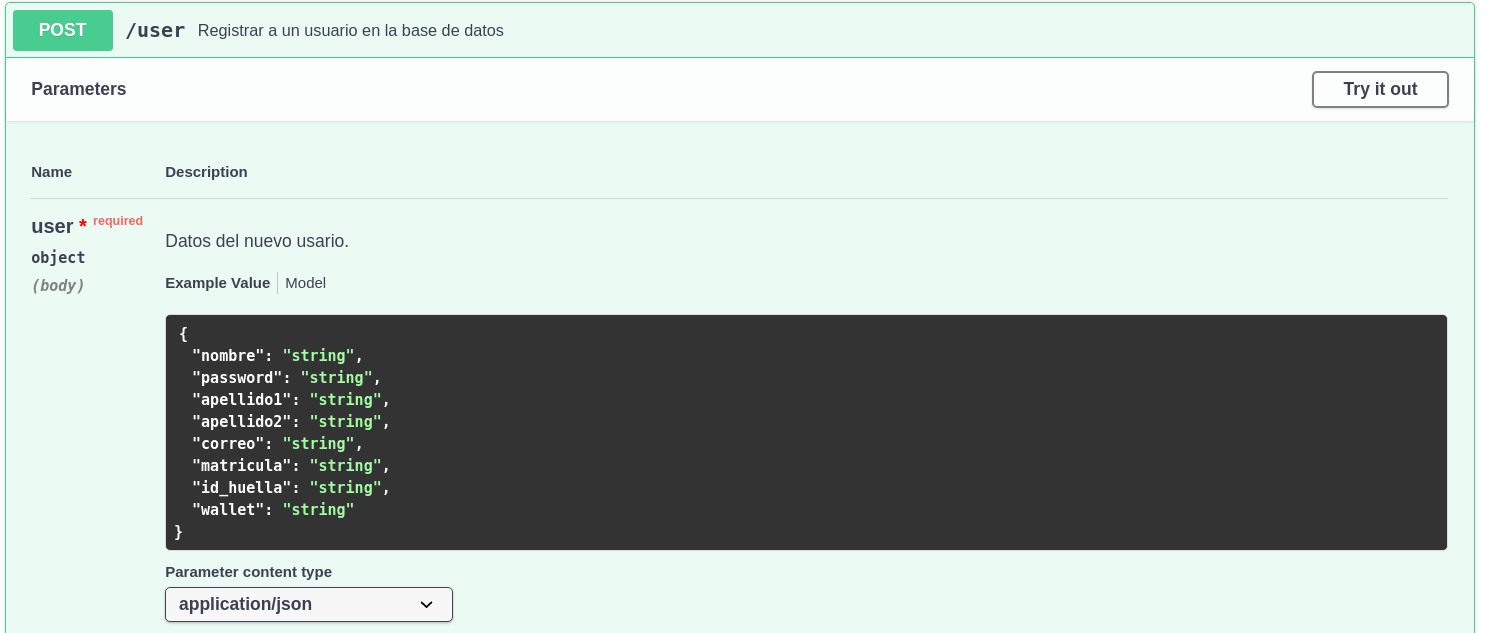
\includegraphics[width=1\linewidth]{figs/Desarrollo/SwaggerUsuario}
  \caption[Swagger Usuario]{Fragmento de documentación de crear usuario}
  \label{fig:swaggerUsuario}
\end{figure}


% --------------------------------------------------
\subsubsection{NodeJS}
Node.js\cite{nodejs} es un entorno de ejecución de \textbf{JavaScript} construido con el motor de \emph{JavaScript V8 de Chrome}. Esta ideado como un entorno orientado a eventos asíncronos con el que se pueden diseñar aplicaciones escalables en la red. Permite tratar múltiples conexiones simultaneas sin que el programador tenga que preocuparse por la concurrencia. Hoy en día, los modelos de concurrencia usan hilos del sistema operativo y requieren de bloquear procesos para operaciones de lectura y escritura. Los usuarios de NodeJS están libres de preocuparse por el bloqueo del proceso, ya que no existe. De ahí que sea muy propicio desarrollar sistemas escalables con NodeJS, de todos modos aunque NodeJS trabaja sin hilos, se pueden aprovechar múltiples núcleos en su entorno, generando varios procesos. \\

Se ha decidido utilizar NodeJS para desarrollar la API de microservicios pues nos da la seguridad de que responderá correctamente a miles de llamadas simultaneas (siempre y cuando el servidor en el que se este ejecutando pueda con el poder de computo que ello requiere). Por lo tanto, permite estar tranquilos y saber que el sistema no se caerá y podrá dar servicio un largo tiempo. Además, NodeJS junto con su gestor de paquetes \emph{npm} permiten mantener el sistema actualizado con facilidad sin preocupeaciones de problemas de dependencias y paquetes desactualizados o con problemas de seguridad. \\

Algunos ejemplos de grandes proyectos que utilizan NodeJS son:
\begin{itemize}
\item Netflix
\item Trello
\item PayPal
\item LinkedIn
\item Uber
\end{itemize}

% --------------------------------------------------
\subsubsection{Swagger}
A la hora de programar una API, no es solo importante que el código sea correcto y funcione correcta y eficientemente. Sino que también es muy importante la documentación de la API, esto permite a otros programadores poder utilizarla sin preocuparse del código, y sin necesidad de conocer el proyecto. Para ello, se ha utilizado \textbf{Swagger} \cite{swagger}. Swagger es un conjunto de herramientas profesionales y de código abierto las cuales ayudan a diseñar y documentar APIs de forma escalable. Swagger permite hacer varias cosas:
\begin{itemize}
\item Diseñar
\item Desarrollar
\item Documentar
\item Testear
\item Virtualizar
\item Monitorizar
\end{itemize}

Para este proyecto, se han aprovechado principalmente las herramientas de \emph{diseño, desarrollo y documentación}. Con la concentración sobre todo en la comodidad de documentación que tiene al utilizar archivos \emph{YAML} (yaml es un formato de serialización de datos legibles por humanos) para generar una documentación ligera, fácil de entender y muy detallada. 

% --------------------------------------------------
\subsubsection{Funcionalidades de la API de Microservicios}
Las comunicaciones de la API se pueden dividir en los siguientes 3 casos de uso generales \ref{fig:casosUso}:

\begin{figure}[h!]
  \centering
  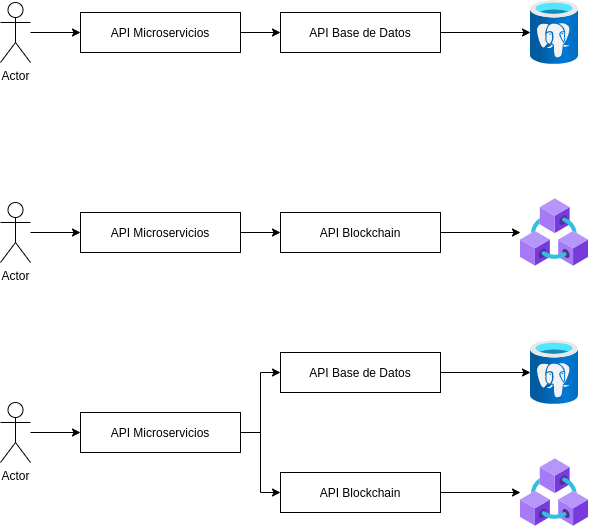
\includegraphics[width=0.6\linewidth]{figs/Desarrollo/UML}
  \caption[Comunicaciones de la API]{Comunicaciones de la API}
  \label{fig:casosUso}
\end{figure}

Siendo más concretos pasemos a listar todas las funcionalidades de las que dispone la API, lógicamente esta no es la documentación completa la cual trae consigo los objetos JSON que aceptan la URIs y los errores u objetos JSON que devuelve cada una de las URIs. En el presente la documentación se mantiene en un repositorio de \emph{gitlab} privado. \\

\begin{center}
  \begin{longtable}{|c|l|m{23em}|}
    \hline
    \textcolor{green}{{\footnotesize POST}} & /user: & Permite registrar a un usuario en la base de datos. \\
    \hline
    \textcolor{blue}{{\footnotesize GET}} & /user/{address}/attendance: & Permite obtener los eventos a los que ha asistido un usuario. \\
    \hline
    \textcolor{blue}{{\footnotesize GET}} & /user/{email}/subscription: & Permite obtener los temas a los que está suscrito un usuario. \\
    \hline
    \textcolor{green}{{\footnotesize POST}} & /login: & Permite iniciar sesión (se comprueba que el usuario exista y se comprueba la contraseña hasheada). \\
    \hline
    \textcolor{green}{{\footnotesize POST}} & /logout: & Permite detectar que un usuario ha cerrado sesión. \\
    \hline
    \textcolor{green}{{\footnotesize POST}} & /subscription: & Permite a un usuario suscribirse a un tema. \\
    \hline
    \textcolor{red}{{\footnotesize DELETE}} & /subscription: & Permite a un usuario desabonar su suscripción de un tema. \\
    \hline
    \textcolor{blue}{{\footnotesize GET}} & /topic: & Permite obtener la lista de temas disponibles. \\
    \hline
    \textcolor{blue}{{\footnotesize GET}} & /topic/{id}/event: & Permite obtener un listado de los eventos de un tema concreto. \\
    \hline
    \textcolor{blue}{{\footnotesize GET}} & /topic/{id}/subscription: & Permite obtener un listado con las suscripciones de un tema. \\
    \hline
    \textcolor{green}{{\footnotesize POST}} & /event: & Permite obtener los datos de la transacción de crear un evento, esta es firmada por el usuario a través de la aplicación Móvil y después enviada a la red blockchain.  \\
    \hline
    \textcolor{blue}{{\footnotesize GET}} & /event/{id}: & Permite obtener los datos de un evento. \\
    \hline
    \textcolor{orange}{{\footnotesize PUT}} & /event/{id}: & Permite obtener los datos de la transacción para modificar un evento, también se firma y envía desde el móvil a la red blockchain.  \\
    \hline
    \textcolor{blue}{{\footnotesize GET}} & /event/{id}/delete/{organizer}: & Permite obtener los parámetros de la transacción para cerrar un evento, se firma y envía desde el móvil. \\
    \hline
    \textcolor{blue}{{\footnotesize GET}} & /eventCatalog: & Permite obtiene un listado con los tipos de eventos.  \\
    \hline
    \textcolor{green}{{\footnotesize POST}} & /event/{id}/validator: & Permite añadir a un nuevo validador a un evento. \\
    \hline
    \textcolor{blue}{{\footnotesize GET}} & /event/{id}/validator/{organizer}: & Permite obtener un listado con los validadores de un evento.  \\
    \hline
    \textcolor{green}{{\footnotesize POST}} & /event/{id}/attendance: & Permite obtener los parámetros de la transacción para registrar la asistencia a un evento, igual que antes, se firma y envía desde el móvil.  \\
    \hline
    \textcolor{blue}{{\footnotesize GET}} & /event/{id}/attendance: & Permite obtener la lista de asistencias a un evento.  \\
    \hline
  \end{longtable}
\end{center}

Gracias a usar swagger, la API sigue la documentación de forma estricta, es decir, no acepta llamadas en las que no se envien los parámetro especificados en la documentación. Si para crear un usuario se requiere de un campo ``email'', si este campo no existe al hacer la llamada a la API, swagger se encarga de rechazar la llamada con un error de formato. Así se logra evitar que el backend tenga errores por variables indefinidas, nulas, o se guarden datos vacíos\dots

